%
% File naaclhlt2013.tex
%

\documentclass[11pt,letterpaper]{article}
\usepackage{naaclhlt2013}
\usepackage{times}
\usepackage{latexsym}
\setlength\titlebox{6.5cm}    % Expanding the titlebox

%add by xiaofan
\usepackage{hyperref}
\usepackage{float}
\usepackage{multirow}
\usepackage{graphicx}
\usepackage{amsmath}
\usepackage{amsfonts}
\usepackage{lipsum} % for the mock text
\usepackage{mdframed}

\title{Twitter sentiment analysis with SVM and RNTN 
\thanks{This is the final project report for CS 388 Natural Language Processing at The University of Texas at Austin in  2014 Spring}}
\author{Yun Wu \qquad Qiren Chen \qquad Xiaofan Lu \\
  University of Texas at Austin \\
 Computer Science Department \\
  {\tt \{ywu, qiren, xiaofan\}@cs.utexas.edu} \\}

\date{}

\begin{document}
\maketitle


\begin{abstract}
\vspace{-3mm}
    In this project, we address the issue of sentiment analysis of twitter messages. 
    We collect three corpora from different domains and propose several pre-processing steps based on the nature of the corpus.    
Features based model and      
Recursive Neural Tensor Network (RNTN) 
are evaluated by extensive experiments. 
Experiment results indicate that RNTN model works better on well formatted text and feature-based model performs better on general topic tweet. 
To the best of our knowledge, this is the first work on twitter sentiment analysis which accounts sentence structure. 
\end{abstract}
\section{Introduction}

Microblogging websites (such as Twitter, Weibo) have gained popularity in recent years. People can easily post real time, short message to express their opinions. 
Sentiment of microblog is of particular interest because such information is valuable in diverse areas such as entertainment, politics and economics.

However, sentiment analysis over twitter message is a challenging task due to the noisy nature of tweet. 
It contains ungrammatical sentences, typos, creative punctuation, slang, new words, URLs, and genre-specific terminology and abbreviations, such as, RT for “re-tweet”, \#hashtags, @mentions. 

Most of existing works of sentiment analysis are based on bag of words classifiers. Different features to improve the performance of bag-of-words model have been proposed\cite{Agarwal:2011}. Such classifiers can work well in longer documents by relying on a few words with strong sentiment such as "great" or "awesome". However, bag-of-words models have difficulties in handling in negation and comparisons, which relies on the structure of sentence. 

Recursive Neural Tensor Network (RNTN) model is recently proposed to capture the compositional effects with higher accuracy. Recursive Neural Tensor Networks take as input phrases of any length. They represent a phrase through word vectors and a parse tree and then compute vectors for higher nodes in the tree using the same tensor-based composition function. \cite{Socher:2013}. The authors claim that RNTN can accurately captures the sentiment change and scope of negation. However, the data set used in the above paper is a bunch of single sentences extracted from well formatted movie reviews, which is quite different from twitter message. We also explore the possibility of domain adaptation of RNTN sentiment model. 

In this paper, we evaluate both bag-of-word model and RNTN model on twitter message to compare the performance of both models. We collect twitter message from different sources and labeled some of them. Such corpus has been pre-processed according to the natural of different models. Experiment results indicates that RNTN perform significantly better on well formatted movie reviews than SVM. When training on \textit{Sentiment Treebank} and testing on general topic tweet, RNTN still perform slightly better. However, due the lack the annotated training set on twitter message, existing RNTN model fails outperform in SVM on the task of sentiment detecting on general topic tweet. 


The paper is organized as follows. Section 2 defines the task we are solving and explains our approach. 
Section 3 presents and discusses experiment results. Section 4 details related work and Section 5 concludes the paper.

\section{Problem Definition and Algorithm}
\label{sec:def}

\subsection{Task Definition}
In this paper, we address the problem of sentiment analysis of Twitter message. To be more precise, 
given a message, we want to classify whether the message is of positive or negative (binary decision), or neutral sentiment (ternary decision). For messages conveying both a positive and negative sentiment, whichever is the stronger sentiment should be chosen. For the following two example messages, we are expected to return positive on the first one and negative on the second. 
\begin{mdframed}[
  leftmargin=\parindent,
  rightmargin=\parindent,
  skipabove=\topsep,
  skipbelow=\topsep
  ]
  If u haven't seen \#Rio2 yet-GO! You need to meet Gabi! Great singer. Cute. Absolutely hysterical! @KChenoweth \url{pic.twitter.com/kkVBUKjqE3}
\end{mdframed}

\begin{mdframed}[
  leftmargin=\parindent,
  rightmargin=\parindent,
  skipabove=\topsep,
  skipbelow=\topsep
  ]
 The rio 2 has one of the worst soundtracks evvvvaaa. I'm at Alamo @Drafthouse Cinema. @marissanicole11 \url{http://4sq.com/1kKF8qE} 
\end{mdframed}

This is an interesting task because sentiment of Twitter message can be used as a barometer for public mood and opinion in diverse areas such as entertainment, politics and economics. For example, 
it was used to provide information on the temporal dynamic of sentiment in reaction to the debate video between Barack Obama and John McCain\cite{Diakopoulos:2010}. 
There is also a report on "Berkshire Hathaway Stock Rises When Anne Hathaway Makes Headlines"\footnote{\url{http://goo.gl/WlfY1c}/}, which indicates that sentiment toward public figure may have potential influence over stock market. 

However, twitter message presents greater challenges for sentiment analysis than traditional text genres, such as newswire data.  Tweets are within 140 characters, often consists of a few short sentences or even a single sentence. 
The language used is very informal, with creative spelling and punctuation, misspellings, slang, new words, URLs, and genre-specific terminology and abbreviations, such as, RT for “re-tweet” and \#hashtags, which are a type of tagging for Twitter messages. \footnote{\url{http://www.cs.york.ac.uk/semeval-2013/task2/}}


\subsection{Algorithm Definition}
We experiment with two different types of models: The first is the traditional bag-of-word model, namely SVM here. The other is the recently proposed Recursive Neural Tensor Network which works pretty good on movie reviews. As different model has different requirement on pre-processing, we first introduce the models we use and then the pre-processing steps. 

\subsubsection{Pre-processing}
The Twitter language is known as informal and flexible. Such properties will provide information about sentiment and should be processed carefully. As the SVM and RNTN model are build upon two different basic ideas, we need to have different pre-processing step for each model. For SVM, our goal is to maximize the information about sentiment while reduce the sparsity of the feature vector. For RNTN, we try to formalize tweets to well-organized sentences such that Stanford parser can recognize it well.

\begin{description}
\item[General features] First we replace all the remaining HTML entities like ``\&amp;'' to ASCII code ``-''. We also delete the quotes around the whole tweet. Then we transform all the URL address to the keyword ``URL'' and the user names(start with @) to the key word ``target'' to keep the structure of the sentences. Hashtags may contain sentimental information so we simply remove the ``\#'' in the front of the hashtag.
\item[Preprocessing with dictionary] Tweets contain very casual language. One common phenomenon is lengthening word. For example, instead of ``so'', Twitter users may repeat 'o's to express their intense feeling as ``sooo'' or ``sooooooo''. We transform all the lengthening words to three repeated letters like ``sooo''. There are also many misspellings and slangs in Twitter and we use a slang dictionary to formalize it.
\item[Preprocessing for SVM] We extract additional features for SVM and attach ``\_neg'' to negated sentences. Detailed information can be found in Section \ref{svm}.  %2.2.1.

\item[Word Cluster] We also try to reduce feature space with word cluster \cite{Owoputi:2013}. Firstly, we obtain hierarchical word clusters via Brown clustering. The algorithm partitions words into a base set of 1,000 clusters, and induces a hierarchy among those 1,000 clusters with a series of greedy agglomerative merges that heuristically optimize the likelihood of a hidden Markov model with a one-class-per-lexical-type constraint. Then we sort the word in each cluster with frequency and use the most frequent one to represent the sentiment of the cluster.


\item[Preprocessing for RNTN] Since RNTN is based on Stanford parser, we need to preserve the structure of sentences while filtering out noisy. 
 Emoticons, for example, can not be easily organized by our parser but provide sentimental information. We split each emoticon with hat, eyes, nose and mouth and replace it with the corresponding adverb. For instance, ``:-)'' will be replaced with ``happily'', ``:O'' with be substituted as ``surprisedly''.  To reduce errors in sentence splitter, multiple punctuation like ``!!!!'' will be shortened to ``!''.  A period is added to each tweet that does not end with punctuation.

%\begin{verbatim}
%^001010110 never neva nvr nevr #never neverr nver neverrr nevaa neeever nevet neeeever nevva
%\end{verbatim}
%
%But it also integrates antonyms, which is fatal for our task.
%\begin{verbatim}
%^111100010011 sad blessed frightening sad lucky frustrating helpful impressed low steady :((( d&d busy
%\end{verbatim}
\end{description}


\subsubsection{SVM}
\label{svm}
A Support Vector Machine (SVM) is a discriminative classifier formally defined by a separating hyperplane. In other words, given labeled training data (supervised learning), the algorithm outputs an optimal hyperplane which categorizes new examples. We use the SVM$^{\text{libSVM}}$ software with a linear and Radial Basis Function (RBF) kernel. We input two sets of vectors of size $m$. Each entry in the vector corresponds to the presence of a feature. For example, with a unigram feature extractor, each feature is a single word found in a tweet. If this single word also appears in our dictionary, the value is $1$, otherwise the value is $0$. In our experiment, we evaluate several different methods to stand for the presence of one feature. 



\newpage

\subsubsection{RNTN}
In Recursive Neural Tensor Network, each word is represented as a $d-$dimensional vector. When an $n-$gram is given to the compositional models, it is parsed into a binary tree (as in Figure \ref{trigram}). We compute the parent vector in a bottom up fashion using a compositionally function $g$ and use node vectors as features for a classifier at that node. 
\begin{figure}[H]
\begin{center}
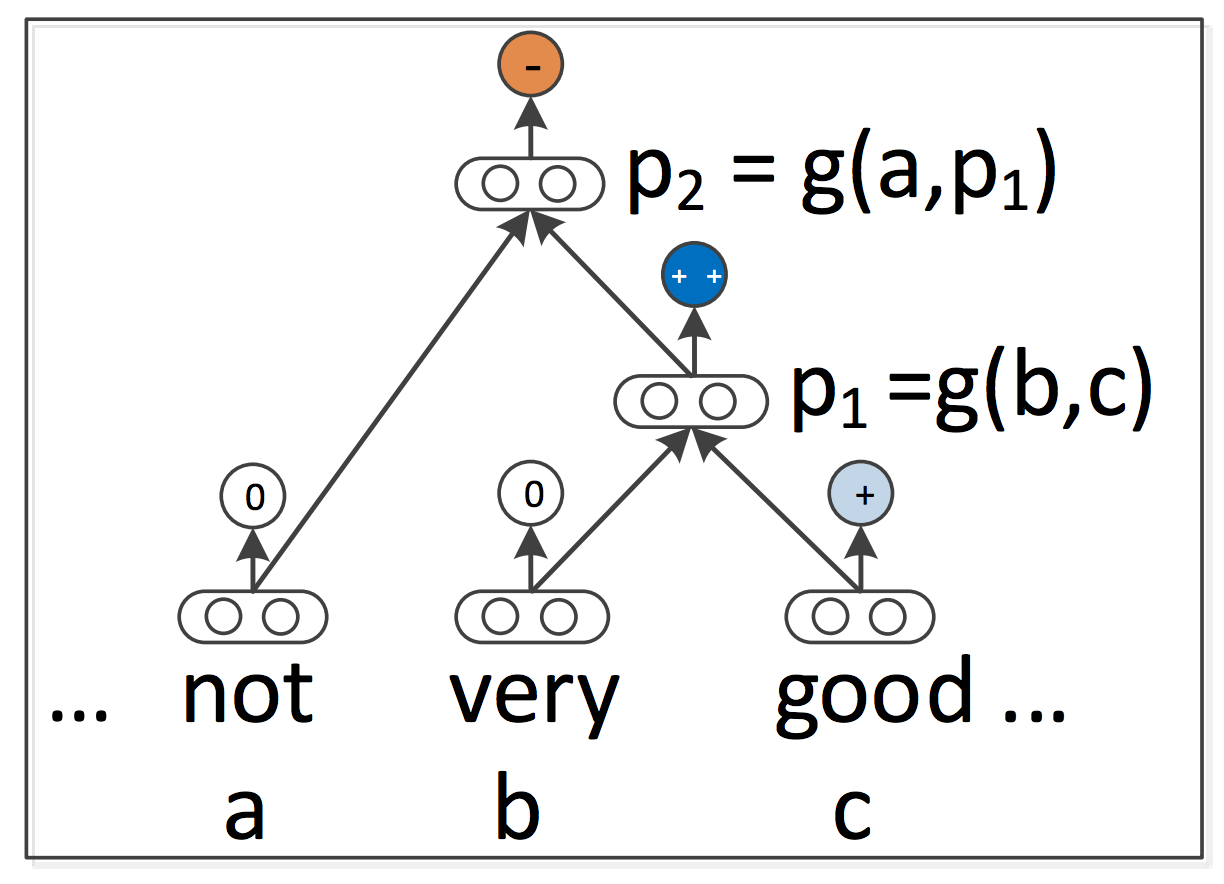
\includegraphics[width = 0.45\textwidth]{pic/trigram.png}
\caption{\label{trigram}Trigram Example (Socher et al., 2013) }
\end{center}
\end{figure}

RNTNs use the following equations to compute the parent vectors: 
\begin{equation*}
p_1 = f \left(  
\begin{bmatrix}
b \\ c
\end{bmatrix}^T
V^{[1:d]} 
\begin{bmatrix}
b \\ c
\end{bmatrix}
+ W
\begin{bmatrix}
b \\ c
\end{bmatrix}
 \right)
\end{equation*}
 
where $f = \textrm{tanh}$ is standard element-wise nonlinearity. $V^{[1:d] \in \mathbb{R}^{2d \times 2d \times d}}$ is the tensor that defines mulitiple bilinear forms. $W \in \mathbb{R}^{d \times 2d}$ is the main parameter to learn. 

The next parent vector $p_2$ in the tri-gram will be computed with the same weights:
\begin{equation*}
p_2 = f \left(  
\begin{bmatrix}
a \\ p_1
\end{bmatrix}^T
V^{[1:d]} 
\begin{bmatrix}
a \\ p_1
\end{bmatrix}
+ W
\begin{bmatrix}
a \\ p_1
\end{bmatrix}
 \right)
\end{equation*}

As we use the RNTN model as a black box in this project, so I skip the details on how to train the model. Interested reader could refer to the paper by Socher et al,. (2013). 



%<<<<<<< HEAD
%=======
%\begin{description}
%\item[General features] First we replace all the remaining HTML entities like ``\&amp;'' to ASCII code ``-''. We also delete the quotes around the whole tweet. Then we transform all the URL address to the keyword ``URL'' and the user names(start with @) to the key word ``target'' to keep the structure of the sentences. Hashtags may contain sentimental information so we simply remove the ``\#'' in the front of the hashtag.
%\item[Preprocessing with dictionary] Tweets contain very casual language. One common phenomenon is lengthening word. For example, instead of ``so'', Twitter users may repeat 'o's to express their intense feeling as ``sooo'' or ``sooooooo''. We transform all the lengthening words to three repeated letters like ``sooo''. There are also many misspellings and slangs in Twitter and we use a slang dictionary to formalize it.
%\item[Preprocessing for SVM] We extract additional features for SVM and attach ``\_neg'' to negated sentences. Detailed information can be found in Section \ref{svm}.  %2.2.1.
%\item[Preprocessing for RNTN] Since RNTN is based on Stanford parser, it may not be good at unknown words or incomplete sentences. Emoticons, for example, can not be organized but provide sentimental information. We split each emoticon with hat, eyes, nose and mouth and replace it with the corresponding adverb. For instance, ``:-)'' will be replaced with ``happily'', ``:O'' with be substituted as ``surprisedly''. Multiple punctuation like ``!!!!'' will be shortened to ``!''. To avoid errors in sentence splitter,  a period is added to each tweet that does not end with punctuation.
%\item[Word Cluster] We also try to reduce feature space with word cluster \cite{Owoputi:2013}. Firstly, we obtain hierarchical word clusters via Brown clustering. The algorithm partitions words into a base set of 1,000 clusters, and induces a hierarchy among those 1,000 clusters with a series of greedy agglomerative merges that heuristically optimize the likelihood of a hidden Markov model with a one-class-per-lexical-type constraint. Then we sort the word in each cluster with frequency and use the most frequent one to represent the sentiment of the cluster. According to our experiment, word cluster does help with nonstandard expressions like 
%
%\begin{verbatim}
%^001010110 never neva nvr nevr #never neverr nver neverrr nevaa neeever nevet neeeever nevva
%\end{verbatim}
%
%But it also integrates antonyms, which is fatal for our task.
%\begin{verbatim}
%^111100010011 sad blessed frightening sad lucky frustrating helpful impressed low steady :((( d&d busy
%\end{verbatim}
%
%
%
%\end{description}
%%>>>>>>> FETCH_HEAD


%Describe in reasonable detail the algorithm you are using to address this problem. A psuedocode description of the algorithm you are using is frequently useful. Trace through a concrete example, showing how your algorithm processes this example. The example should be complex enough to illustrate all of the important aspects of the problem but simple enough to be easily understood. If possible, an intuitively meaningful example is better than one with meaningless symbols. 



%\section{Pre-processing}
\subsection{Twitter related features}
\subsection{Slang Translation}
\subsection{Emoticons}
\subsection{Spelling Correction}
\subsection{Word Cluster}
\section{Experiment}
\label{sec:exp}


\subsection{Corpus}
We conduct our experiments on three types of corpus.
\begin{itemize}
\item  The first corpus is the Stanford sentiment treebank released by Socher et. al. (2013). It is based on the dataset introduced by Pang and Lee (2005) and consists of 11,855 single sentences extracted from movie reviews on \url{http://www.rottentomatoes.com/}. It was parsed with the Stanford parser (Klein and Mannning, 2003) and includes a total of 215,154 unique phrases from those parse trees, each annotated by 3 human judges. To the best of our knowledge, it is the only public available corpus upon which a RNTN sentiment model can be trained right now. We refer to this corpus by \textit{Sentiment Treebank} in the reset of paper. 

\item  The second corpus is movie reviews on Twitter. We have 364 tweets extracted from two specialized review accounts (@FilmReviewIn140, @MovieTwoosh). Such reviews are mostly well formatted, usually consist of several sentences. The author rated each movie with A to F grades and the label the sentiment of the tweet base on the grade. Tweets with a grade no worse than B are labeled positive otherwise negative.  We refer to this corpus by \textit{moive} in the reset of paper. 

\item The third corpus is general tweet message. It is taken from SemEval-2013: Sentiment Analysis in Twitter Task B\footnote{\url{http://www.cs.york.ac.uk/semeval-2013/task2/index.php?id=data}}. In their release, each of the tweet messages has been manually labeled as positive, negative, or neutral. Out of all the 5,750 messages, 2,042 are positive, 855 are negative and 2853 are neutral.  We refer to this corpus by \textit{SemEval} in the reset of paper. 
\end{itemize}

\subsection{Single Sentence Sentiment}
We firstly evaluate both models using \textit{Sentiment Treebank}, The same training/testing splits as in the original paper\cite{Socher:2013} is used. 

\begin{table}[H]
  \begin{center}
    \begin{tabular}{cccc}\hline
      \multirow{2}{*}{Model} 
      & \multicolumn{3}{c}{Accuracy} \\\cline{2-4}
    & positive & negative & overall \\ \hline
    RNTN  & 80.83      &   87.91   &  84.27      \\ 
    SVM$_S$  & 74.15      &  73.79    &    73.97     \\ 
    SVM$_L$  & 75.90      & 73.90         &   74.90      \\ \hline
    \end{tabular}
    \end{center}
    \caption{\label{exp_1} Binary decision}
\end{table}

In SVM$_S$, we use a smaller dictionary (1635 words) in which words appear more than 10 times are used. In SVM$_L$, we build a larger dictionary (3504 words) with the bar lowered to 5 times. 

As we can see from Table \ref{exp_1}, the performance of RNTN model is significantly better than SVM models. This is consistent with the result of the original paper\cite{Socher:2013}. The huge boost comes from the fact that the structure of the sentence is utilized in the RNTN model. It might seems to be an unfair comparison as more information is needed (the sentiment of each parse of the sentence) in training the RNTN model. 
However, even if we train the SVM model with sentiment label of each parse as well, the result won't improve much as what SVM sees is just a subset of the original bag.  


\subsection{Multiple Sentences Sentiment}
We then evaluate how to combine the sentiment of multiple sentences. This is not an issue of SVM because only a larger bag is needed. However, RNTN relies on the structural of single sentence so we need to combine the sentiment from multiple sentences within a single tweet. Here, we train the model on \textit{Sentiment Treebank} and test it on \textit{movie} corpus. 

As for the RNTN model, we evaluate two ways to combine the sentiment of the whole tweet (multiple sentences). The first is to make hard (binary) decision on single sentence ( either positive or negative) and sentiment of the tweet is decided by majority vote. Soft information (probability) is only used to break a tie. The second way fully relis on soft (probability) information. For each sentence, we generate a 5-element vector for the probability of the having the corresponding sentiment (very negative, negative, neutral, positive, very positive). We add the vector for all the sentences together and make final decision based on the combined vector. 
\begin{table}[H]
  \begin{center}
    \begin{tabular}{cccc}\hline
      \multirow{2}{*}{Model} 
      & \multicolumn{3}{c}{Accuracy(\%)} \\\cline{2-4}
    & positive & negative & overall \\ \hline
    RNTN$_{hard}$  & 70.08 	    &  81.54       &  74.18     \\
    RNTN$_{soft}$  & 78.21     &   80.0	    &   78.85    \\ 
    SVM           & 73.50     &   66.92     &   71.15      \\\hline 
    \end{tabular}
    \end{center}
    \caption{\label{exp2_1} Binary decision}
\end{table}

From Table \ref{exp2_1}, we can see that both RNTN models perform better than SVM. For the two RNTN models, 
 hard decision model has worse performance than soft decision in positive sentiment but slightly better on negative sentiment. This indicates that RNTN model tend to label a sentence as negative. Soft combining outperforms hard combining by more than 4\% in the overall result. This is reasonable because more information is available in soft decision combining. Based on the above result, we use soft mode in the following experiments. 

%\subsection{Effect of Preprocessing}
%We also evaluates how much preprocessing contributed to our final performance. In this experiment, we still use the model trained on \textit{Sentiment Treebank} but tested on \textit{movieB} corpus, which contains noisy common twitter message collected by searching movie names. We evaluated both models with and without preprocessing the original corpus. 
%
%\begin{table}[H]
%  \begin{center}
%    \begin{tabular}{ccc}\hline
%      \multirow{2}{*}{Model} 
%      & \multicolumn{2}{c}{Overall Accuracy(\%)} \\\cline{2-3}
%    & with pre-processing & w/o pre-processing \\ \hline
%    RNTN  &          &     	       \\ 
%    SVM1  & ~        &              \\ 
%    SVM2  & ~        &              \\ \hline
%    \end{tabular}
%    \end{center}
%    \caption{\label{exp5_3} Effect of preprocessing}
%\end{table}
%
%Comparing both table, we can see that preprocessing indeed helped in improving the performance.  
\vspace{-5pt}
\subsection{General topic Tweet}
We conducted three sets of experiment over the general topic twitter corpus \textit{SemEval}. 
\begin{itemize}
\item Exp 1: Training on 90\% of \textit{SemEval} and testing on the rest 10\%. 
This is the classic experiment setup. However, as we don't have annotated sentiment parse tree  (the sentiment of each node of the parse tree, which is required to train the RNTN model), a RNTN model based on \textit{SemEval} can not be trained. Thus, we evaluate the following features of SVM model in this experiment. 

\begin{enumerate}
\item Word unigram and bigram (Unigram or Bigram): In our experiment, we try to use the presence or absence of contiguous sequences of tokens as a feature. We use unigram and bigram as features and evaluate the different performance. Also we use three different methods to present unigram feature. \\
 \textbf{Bianry Format}: if the word is present in the Tweet, we use $0/1$ to show presence of a word.\\ 
 \textbf{Frequency}: The count of each word is used as unigram feature. For example, if “good” appears twice in the Tweet, we set 2 to this word.\\
 \textbf{tf-idf}: It is a numerical statistic that is intended to reflect how important a word is to a document in a collection or corpus. tf-idf is the product of two statistics, term frequency and inverse document frequency. 
  \begin{eqnarray*}
      tfidf_{i,j} = & tf_{i,j} \times idf_{i} & \qquad \text{where} \\
      tf_{i,j} = & \frac{n_{i,j}}{\sum_k n_{k,j}} & \\
      idf_i = & \log \frac{|D|}{|\{j: t_i \in d_j\}|} &
  \end{eqnarray*}   
  
  	\item Elongated word (\textbf{-elongated}): Lengthening words by repeating letters (such as “coooool”, “goooood”) is reported to be an strong indication of sentiment. Brody et al. (2011) reported that on average, one out of six sentences has word lengthening. In our experiment, we also take elongated word as a feature. 
   \item Targets, Hashtags, URLs, Numbers (\textbf{-url-num}): These are the features related to Twitter. Users of Twitter use the “\@” symbol to refer to other users in this manner automatically alerts them. Users use hashtags “\#” to mark topics. 
  	%This is primarily done to increase the visibility of their tweets. URL and numbers are common in tweet. 
   \item Negation (-\textbf{neg}): The effect of negation word is not simply the opposite of the original sentiment. In this paper, we try to append a NEG suffix to every word appearing between a negation and a clause-level punctuation mark. 
  
\end{enumerate}


\begin{table}[H]
  \begin{center}
    \begin{tabular}{llc}\hline
     \multicolumn{2}{c}{Feature} & Accuracy (\%)     \\\hline
     \multirow{3}{*}{Unigram}    & Binary feature  &  78.84  \\ 
                                 & Frequency       &  78.64  \\ 
                                 & Tf-idf          &  78.22 \\
     \multicolumn{2}{l}{Bigram}                    &  70.41 \\  
     \multicolumn{2}{l}{Unigram-Bigram}            &  78.26 \\         
     \multicolumn{2}{l}{Unigram-url-num}           &  \textbf{79.32} \\
     \multicolumn{2}{l}{Unigram-elongated}         &  79.01 \\
     \multicolumn{2}{l}{Unigram-url-num-elongated} &  79.19 \\
     \multicolumn{2}{l}{Unigram-neg}               &  78.77 \\
     \multicolumn{2}{l}{Unigram-neg-url-num}       &  78.19 \\
     \multicolumn{2}{l}{Unigram-neg-enlongated}    &  78.34 \\
     \multicolumn{2}{l}{Unigram-neg-url-num-enlongated}  &  77.95 \\\hline      
    \end{tabular}
    \end{center}
    \caption{\label{exp5_1} Experiment 1}
\end{table}

\item Exp 2: Training on \textit{Sentiment Treebank} and testing on \textit{SemEval}. \\ 
In this experiment, we apply the model trained on \textit{Sentiment Treebank} on the general topic twitter message. It may sounds wired but as we mentioned earlier, \textit{Sentiment Treebank} is the only corpus upon which we can train RNTN model. To be fair, we train a SVM model in the same way and compare the performance of the two in both binary-decision and ternary-decision task. 
\begin{table}[H]
  \begin{center}
    \begin{tabular}{cccc}\hline
      \multirow{2}{*}{Model} 
      & \multicolumn{3}{c}{Accuracy(\%)} \\\cline{2-4}
    & positive & negative & overall \\ \hline
    RNTN  & 69.83     &   70.17	    &   69.93    \\ 
    SVM   & 67.14     &   60.91     &   65.30      \\ \hline
    \end{tabular}
    \end{center}
    \caption{\label{exp5_2_1} Experiment 2.1}
\end{table}

\begin{table}[H]
  \begin{center}
    \begin{tabular}{ccccc}\hline
      \multirow{2}{*}{Model} 
      & \multicolumn{4}{c}{Accuracy(\%)} \\\cline{2-5}
    & positive & negative & neutral & overall \\ \hline
    RNTN  & 48.12    &   43.17  	   &   49.40       & 48.02    \\ 
    SVM   & 52.52    &   23.86     &   44.69       & 37.14    \\ \hline
    \end{tabular}
    \end{center}
    \caption{\label{exp5_2_2} Experiment 2.2}
\end{table}

From Table \ref{exp5_2_1} and Table \ref{exp5_2_2}, we can see that RNTN out perform SVM in both binary decision and ternary decision. However, the performance is worse than the result from Table \ref{exp5_1}. 

The huge decrease in SVM model resulted from the difference of the two corpus. 
Clearly, twitter specific feature helps SVM model a lot but such feature is not available in the \textit{Sentiment Treebank}. 

Another interesting comparison is the performance of RNTN in Table \ref{exp_1} and Table \ref{exp5_2_2}. Like statistical parser, RNTN model is also quite specific to the genre of the training corpus. To make the problem worse, the Stanford parse doesn't work quite well on twitter message due to the noisy nature of it. 

\item Exp 3: Domain adaptation of RNTN\\
In this experiment, we explore domain adaptation of RNTN sentiment model. This is an interesting experiment as gathering fully annotated training data on twitter message is expensive and labor intensive. We have fully annotated corpus in \textit{Sentiment Treebank} but \textit{SemEval} is only been labeled positive, neutral or negative. In this experiment, we first train the model on \textit{Sentiment Treebank}, then use the above model to label the training set of \textit{SemEval} in sentiment treebank format. We retrain the model with both \textit{Sentiment Treebank} and the labeled  training set of \textit{SemEval}. In the end, we test the new model on the test set of \textit{SemEval}.


%\begin{table}[H]
%  \begin{center}
%    \begin{tabular}{cccc}\hline
%      \multirow{2}{*}{Model} 
%      & \multicolumn{3}{c}{Accuracy(\%)} \\\cline{2-4}
%    & positive & negative & overall \\ \hline
%    RNTN  &          &     	   &      \\ 
%    SVM1  & ~        &          &         \\ 
%    SVM2  & ~        &          &         \\ \hline
%    \end{tabular}
%    \end{center}
%    \caption{\label{exp5_3_1} Experiment 3.1}
%\end{table}


%\begin{table}[H]
%  \begin{center}
%    \begin{tabular}{ccccc}\hline
%      \multirow{2}{*}{Model} 
%      & \multicolumn{4}{c}{Accuracy(\%)} \\\cline{2-5}
%    & positive & negative & neutral & overall \\ \hline
%    Binary  & ~        &   ~	   &   --         &    \\ 
%    Ternary  & ~        &          &             &   \\ \hline
%    \end{tabular}
%    \end{center}
%    \caption{\label{exp5_3} Experiment 3}
%\end{table}

\begin{figure}[H]
\begin{center}
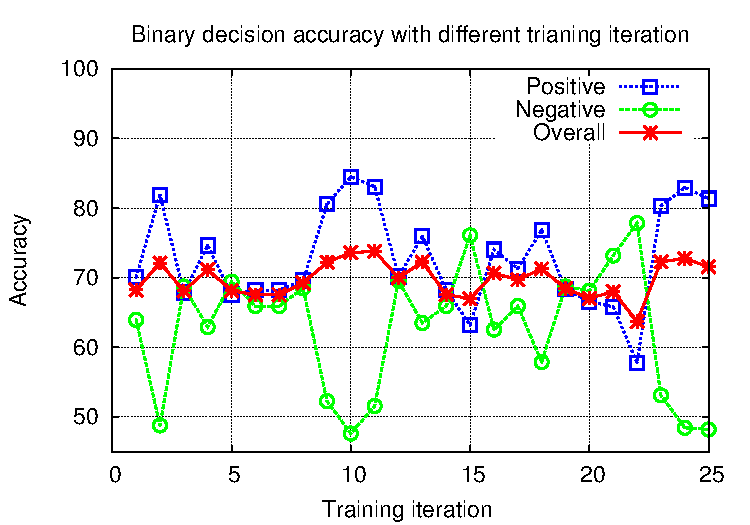
\includegraphics[width = 0.5\textwidth]{pic/model_2b.pdf}
\caption{Binary decision }
\end{center}
\end{figure}

\begin{figure}[H]
\begin{center}
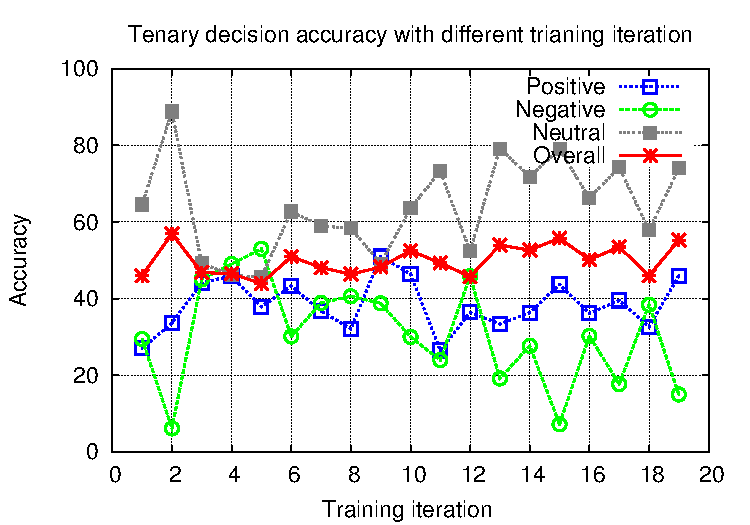
\includegraphics[width = 0.5\textwidth]{pic/model_3c.pdf}
\caption{Ternary decision }
\end{center}
\end{figure}

We train the model with different iterations and evaluate all the models. As we can see from the above two figures, the result fluctuates a lot. Unfortunately, we don't see significant improvement in performance with domain adaptation.  
\end{itemize}


\subsection{Discussion}
\subsubsection{SVM}
We explore the usage of n-gram combined with other features. 
\begin{itemize}
\item \textbf{Unigram}: Experiment results show that use binary format to present unigram performs best. The result of using frequency and Tf-idf to present unigram is slightly worse than using binary format, but almost the same. The reason for this is Tweet is rather short (at most 140 characters). One word is hardly to appear twice in one Tweet. So frequency is not an obviously good feature in Tweets as in other corpus. For Tf-idf, because there are so many topics in Tweets, each word is hardly used to distinguish sentiment.

\item \textbf{Bigram}: We use bigrams to help with tweets that contain negated phrases like “not good” or “not cool”. In our experiments, Bigram as a feature does not improve accuracy. However, bigrams tend to be very sparse and the size of our corpus is relatively small. So bigram doesn’t work well on Twitter sentiment analysis. As we can see, the overall accuracy drops. In general using bigrams as features is not helpful because the feature space is very sparse. Thus we want to combine Unigram and Bigram as features. 

\item \textbf{Unigram-Bigram}: Results show Unigram-Bigram as a feature doesn’t help. Compared to Unigram features, accuracy drops from 78.84\% to 78.26\%. For Alec Go (2009), there was also a decline for Unigram-Bigram as features. 

\item \textbf{Targets, Hashtags, URLs, Numbers}: The feature combining URL, Numbers with Unigram performs best in our experiment. The result shows that the number of URLs and Numbers is helpful for this task. 

\item \textbf{Elongated}:  Elongated word as a feature doesn’t help. The reason is that we can hardly classify different elongated forms of one word into one classification, such as “goood” and “gooooddddd”. So elongated words as a feature are sparse and hardly provide other information. In the future work, if we have a better algorithm to deal with elongated words, we can improve the results. 

\item \textbf{Negations}: Negations as features work almost as well as Unigram as a feature. The reason why negations don’t improve the results is that it makes the dictionary larger than the original one. But since the size of corpus is relatively small, so negations don’t show its advantage in our experiment. 

\end{itemize}








\section{Related Work}



\section{Future work}
\label{sec:future}
\begin{itemize}
\addtolength{\itemsep}{-0.5\baselineskip}

\item Better pre-processing technique \\
Due to the noisy nature of twitter messages, how well we can preprocess it matters a lot. How to preserve the structure of the original sentence and filter out unnecessary information is a challenging task. 

\item Better parser for twitter message \\
As the RNTN is built upon parse trees, the performance of the parser is of great importance to RNTN model. However, most of existing parsers, including the one we used (Stanford Parser) are trained on newswire data, which is very different from the twitter messages. We believe within a few years, the focus of the research community on twitter message will shift from current POS tagging to building an accurate parser. 

\item Sentiment treebank over twitter message \\
Our experiments are limited by the fact that there is no labeled sentiment treebank of twitter messages. This is largely because that RNTN model has just come out. Building our own sentiment treebank would be too much for us as a course project. However, it would be of great help if such a sentiment treebank over twitter messages is available to the research community. 


\end{itemize}



\section{Conclusion}
\label{sec:length}
Better parser needed. 

\section*{Acknowledgments}
We would like to thanks Dr. Mooney for his guidance. Thanks researcher who share their tweet corpus. 

% include your own bib file like this:
%\bibliographystyle{acl}
%\bibliography{acl2014}


\begin{thebibliography}{}

%\bibitem[\protect\citename{Aho and Ullman}1972]{Aho:72}
%Alfred~V. Aho and Jeffrey~D. Ullman.
%\newblock 1972.
%\newblock {\em The Theory of Parsing, Translation and Compiling}, volume~1.
%\newblock Prentice-{Hall}, Englewood Cliffs, NJ.
%
%\bibitem[\protect\citename{{American Psychological Association}}1983]{APA:83}
%{American Psychological Association}.
%\newblock 1983.
%\newblock {\em Publications Manual}.
%\newblock American Psychological Association, Washington, DC.
%
%\bibitem[\protect\citename{{Association for Computing Machinery}}1983]{ACM:83}
%{Association for Computing Machinery}.
%\newblock 1983.
%\newblock {\em Computing Reviews}, 24(11):503--512.
%
%\bibitem[\protect\citename{Chandra \bgroup et al.\egroup }1981]{Chandra:81}
%Ashok~K. Chandra, Dexter~C. Kozen, and Larry~J. Stockmeyer.
%\newblock 1981.
%\newblock Alternation.
%\newblock {\em Journal of the Association for Computing Machinery},
%  28(1):114--133.
%
%\bibitem[\protect\citename{Gusfield}1997]{Gusfield:97}
%Dan Gusfield.
%\newblock 1997.
%\newblock {\em Algorithms on Strings, Trees and Sequences}.
%\newblock Cambridge University Press, Cambridge, UK.


\bibitem[\protect\citename{Socher \bgroup et al.\egroup}2013]{Socher:2013},
Socher, Richard  and  Perelygin, Alex  and  Wu, Jean  and  Chuang, Jason  and  Manning, Christopher D.  and  Ng, Andrew Y.  and  Potts, Christopher. 
\newblock 2013. 
\newblock Recursive Deep Models for Semantic Compositionality Over a Sentiment Treebanka
\newblock {\em Proceedings of the 2013 Conference on {E}mpirical {M}ethods in {N}atural {L}anguage {P}rocessing} 

\bibitem[\protect\citename{Diakopoulos and Shamma} 2010]{Diakopoulos:2010},
N. Diakopoulos, D. A. Shamma. 
\newblock April, 2010.
\newblock Characterizing Debate Performance via Aggregated Twitter Sentiment.
\newblock {\em Conference on Human Factors in Computing Systems (CHI). }

\bibitem[\protect\citename{Agarwal \bgroup et al.\egroup}2011]{Agarwal:2011},
Apoorv Agarwal, Boyi Xie, Ilia Vovsha, Owen Rambow, and Rebecca Passonneau. 
\newblock 2011. 
\newblock Sentiment analysis of Twitter data. 
\newblock {\em In Proceedings of the Workshop on Languages in Social Media (LSM '11). Association for Computational Linguistics, Stroudsburg, PA, USA, 30-38.}

\bibitem[\protect\citename{Owoputi \bgroup et al.\egroup}2011]{Owoputi:2013},
Olutobi Owoputi and Chris Dyer and Kevin Gimpel and Nathan Schneider and Noah A. Smith. 
\newblock 2013. 
\newblock Improved part-of-speech tagging for online conversational text with word clusters
\newblock {\em In Proceedings of NAACL}



\end{thebibliography}













\end{document}
